\section{Discretisation}\label{sec:discrete}

$l = [0, \hdots, N]$ where 

As done in \cite{Harrison2018}, it is useful to place either $p$ or $v$ on an interleaved grid; both in space and time. Following Harrison, we place $v$ on this interleaved grid. Accordingly, system \eqref{eq:firstOrderSystem} is discretised into the following finite difference scheme (FDS)
\begin{subequations}\label{eq:FDS}
    \begin{align}
        \frac{\bar S_l}{\rho_0 c^2}\delta_{t+}p_l^n &= -\delta_{x-}(S_{l+1/2}v_{l+1/2}^{n+1/2}),\label{eq:discPressure}\\
        \rho_0 \delta_{t-}v_{l+1/2}^{n+1/2}&=-\delta_{x+}p_l^n,\label{eq:discVelocity}
    \end{align}
\end{subequations}



Boundary conditions:

At $l = 0$



after which the update schemes become
\begin{subequations}
    \begin{align}
        p_l^{n+1} &= p_l^n - \frac{\rho_0 c \lambda}{\bar{S}_l}(S_{l+1/2}v_{l+1/2}^{n+1/2}-S_{l-1/2}v_{l-1/2}^{n+1/2}),\label{eq:pressureUpdate}\\
        v_{l+1/2}^{n+1/2} &= v_{l+1/2}^{n-1/2}-\frac{\lambda}{\rho_0 c}(p_{l+1}^n - p_l^n),\label{eq:velocityUpdate}
    \end{align}
\end{subequations}
where $\lambda = ck/h$ is referred to as the Courant number and
\begin{equation}
    \lambda \leq 1
\end{equation}
in order for the scheme to be stable. 

\begin{figure}[ht]
    \centering
    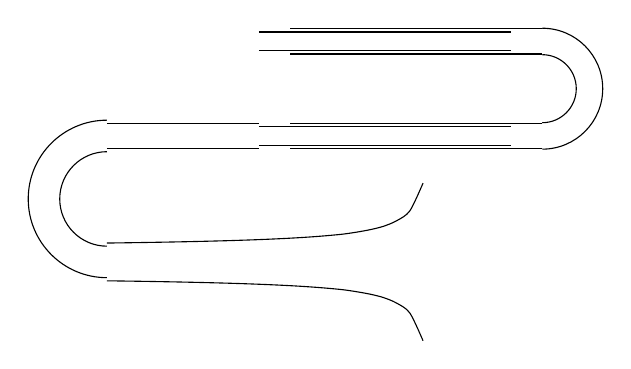
\begin{tikzpicture}[scale = 8]

    \def\hornOffset{0.02};
    \def\stepSize{0.005}

    % tuning slide params
    \def\tuningSlideDim{0.1};
    \pgfmathsetmacro{\tuningSlideRad}{\stepSize + \hornOffset};

    % gooseneck params
    \def\gooseNeckLength{0.241};
    \pgfmathsetmacro{\gooseNeckRad}{\tuningSlideRad - \stepSize};

    % inner slide params
    \def\innerLength{0.4};
    \pgfmathsetmacro{\innerRad}{\gooseNeckRad - \stepSize};

    % outer slide params
    \def\outerLength{\innerLength};
    \pgfmathsetmacro{\outerRad}{\gooseNeckRad};
    \pgfmathsetmacro{\extension}{0.05};

    \def\endOfSlideDim{0.075};
    \pgfmathsetmacro{\endOfSlideRad}{\outerRad * 1.05};

    %% draw horn
    % \filldraw[black] (0, 0) circle (0.1pt) node[anchor=west](origin){\tiny(0, 0)}; 

    \draw[domain=0:0.502, smooth, variable=\x, black] plot ({\x}, {\hornOffset + 0.0063 * ((0.502-\x) + 0.0174)^(-0.7)});
    
    \draw[domain=0:0.502, smooth, variable=\x, black] plot ({\x}, {-\hornOffset-0.0063 * ((0.502-\x) + 0.0174)^(-0.7)});
    
    % draw tuningSlide
    \pgfmathsetmacro{\innerTuningSlideDim}{(\tuningSlideDim - \tuningSlideRad)}
    \pgfmathsetmacro{\outerTuningSlideDim}{(\tuningSlideDim + \tuningSlideRad)}

    % \draw (0, 0) arc(270:90:\tuningSlideDim cm and \tuningSlideDim cm);

    % \filldraw[black] (0, 2*\tuningSlideDim) circle (0.1pt) node[anchor=west](origin){\tiny (0, 0.2)}; 

    \draw (0, \tuningSlideRad) arc(270:90:\innerTuningSlideDim cm and \innerTuningSlideDim cm);

    \draw (0, -\tuningSlideRad) arc(270:90:\outerTuningSlideDim cm and \outerTuningSlideDim cm);

    % draw gooseneck
    \draw (0, 2*\tuningSlideDim + \gooseNeckRad) -- (\gooseNeckLength, 2*\tuningSlideDim + \gooseNeckRad);

    \draw (0, 2*\tuningSlideDim - \gooseNeckRad) -- (\gooseNeckLength, 2*\tuningSlideDim - \gooseNeckRad);

    % draw inner slide
    \draw (\gooseNeckLength, 2*\tuningSlideDim + \innerRad) -- (\gooseNeckLength+\innerLength, 2*\tuningSlideDim + \innerRad);

    \draw (\gooseNeckLength, 2*\tuningSlideDim - \innerRad) -- (\gooseNeckLength+\innerLength, 2*\tuningSlideDim - \innerRad);

    % draw outer slide
    \pgfmathsetmacro{\outerSlideStart}{\gooseNeckLength + \extension};

    \draw (\outerSlideStart, 2*\tuningSlideDim + \outerRad) -- (\outerSlideStart+\outerLength, 2*\tuningSlideDim + \outerRad);

    \draw (\outerSlideStart, 2*\tuningSlideDim - \outerRad) -- (\outerSlideStart+\outerLength, 2*\tuningSlideDim - \outerRad);

    % draw end of slide
    \pgfmathsetmacro{\innerEndOfSlideDim}{(\endOfSlideDim - \endOfSlideRad)};
    \pgfmathsetmacro{\outerEndOfSlideDim}{(\endOfSlideDim + \endOfSlideRad)};

    \pgfmathsetmacro{\startEndOfSlide}{\outerSlideStart + \outerLength};

    \draw (\startEndOfSlide, 2*\tuningSlideDim+\endOfSlideRad) arc(-90:90:\innerEndOfSlideDim cm and \innerEndOfSlideDim cm);

    \draw (\startEndOfSlide, 2*\tuningSlideDim-\endOfSlideRad) arc(-90:90:\outerEndOfSlideDim cm and \outerEndOfSlideDim cm);

    % draw second outer slide

    \draw (\outerSlideStart, 2*\tuningSlideDim + 2 * \endOfSlideDim + \outerRad) -- (\outerSlideStart+\outerLength, 2*\tuningSlideDim + 2 * \endOfSlideDim + \outerRad);

    \draw (\outerSlideStart, 2*\tuningSlideDim + 2 * \endOfSlideDim - \outerRad) -- (\outerSlideStart+\outerLength, 2*\tuningSlideDim + 2 * \endOfSlideDim - \outerRad);

    % draw inner slide
    \draw (\gooseNeckLength, 2*\tuningSlideDim+ 2 * \endOfSlideDim + \innerRad) -- (\gooseNeckLength+\innerLength, 2*\tuningSlideDim+ 2 * \endOfSlideDim + \innerRad);

    \draw (\gooseNeckLength, 2*\tuningSlideDim + 2 * \endOfSlideDim - \innerRad) -- (\gooseNeckLength+\innerLength, 2*\tuningSlideDim + 2 * \endOfSlideDim - \innerRad);

% \begin{scope}[very thick,decoration={
%     markings,
%     mark=at position 0.5 with {\arrow{>}}}
%     ] 
%     \draw[postaction={decorate}] (-4,0)--(4,0);
% \end{scope}
    
    \end{tikzpicture}
    \caption{Lipsystem with the equilibrium at 0 and the distance from the lower lip $H_0$.}
    \label{fig:lipSystem}
\end{figure}